\let\textcircled=\pgftextcircled
\chapter{Background}
\label{chap:background}

\textit{\initial{I}n this chapter, we present basic concepts such as server virtualization, the types of server virtualization systems, \acrshort{numa} architectures and \acrshort{io} mechanism in virtualized environments such as Xen for a better apprehension of the work done. The plan of this chapter is as follows: }

\minitoc

\newpage    
\section{Server virtualization}
Most servers use less than 15\% of their resources \citep{serv1}. Server virtualization addresses these inefficiencies by allowing multiple operating systems to run on a single physical server as virtual machines, each with access to the underlying server's computing resources. To achieve server virtualization, we need a server virtualization system (hypervisor). There are mainly 4 types of server virtualization systems which are: \textbf{full virtualization, para-virtualization, \acrshort{os} level virtualization and hardware assisted virtualization}. Depending on the needs, one type may be better than another. In the next section, we discuss the different types of server virtualization systems and give some examples.

\subsection{Types of server virtualization systems}
\subsubsection{Full virtualization}
Here, the hypervisor is a software that runs on top of the host\footnote{Here we refer to the physical machine} \acrshort{os} as shown on Figure \ref{fig:full-virtualization}. The latter virtualizes/emulates the hardware for the guest \acrshort{os} (virtual machine), and is believed to communicate directly with the hardware. This solution is very similar to an \textbf{emulator}, and sometimes even mistaken for the latter. However, the \acrshort{cpu}, the \acrshort{ram}, as well as the storage memory, are directly accessible to the virtual machines, while on an emulator the \acrshort{cpu} is emuled, and the performance is considerably reduced compared to virtualization.
\paragraph{} This type of server virtualization is offered by software such as \textbf{Virtualbox, VMWare Workstation.} Hypervisors enabling this type of server virtualization are said to be of \textbf{type 2}.

\begin{figure}[!h]
    \centering
    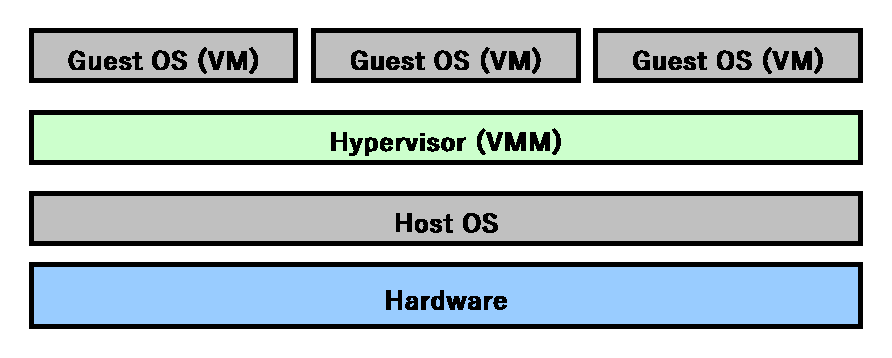
\includegraphics[scale=0.65]{fig02/full-virtualization.pdf}
    \caption{Full virtualization architecture}
    \label{fig:full-virtualization}
\end{figure}

\subsubsection{OS level virtualization}
Here, the hypervisor is called an \textbf{isolator}. An isolator is software that isolates the execution of applications in \textbf{contexts}, or \textbf{execution areas} as shown on Figure \ref{fig:os-level-virtualization} . The isolator thus makes it possible to run the same application several times in a multi-instance mode (several instances of execution) even if it was not designed for that. This solution is very efficient, because of the \textbf{small overhead}, but the virtualized environments are not completely isolated.
\paragraph{} There is a visible performance. However, we can not really talk about virtualization of operating systems. Only connected to Linux systems, isolators are actually made up of several elements and can take many forms. This type of virtualization is offered by software as \textbf{Linux-Vserver, Chroot, BSD Jail, OpenVZ and LXC (Linux Container)}.

\begin{figure}[!h]
    \centering 
    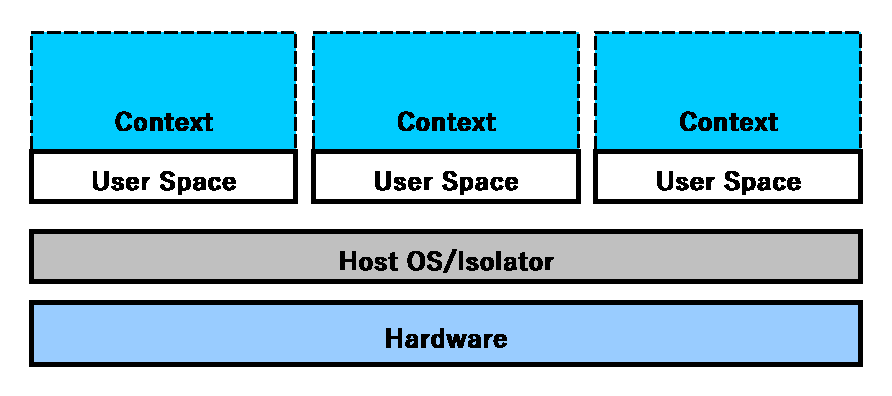
\includegraphics[scale=0.65]{fig02/os-level-virtualization.pdf}
    \caption{OS level virtualization architecture}
    \label{fig:os-level-virtualization}
\end{figure}

\subsubsection{Hardware assisted virtualization}
This is a particular case of server virtualization where the hardware is designed to ease virtualization. Here the virtual machines are called \textbf{Hardware Virtual Machines (HVM)}. The \acrshort{cpu} designers such as \textbf{Intel} and \textbf{\acrshort{amd}} modify the hardware to enable technologies such as \textbf{Intel VT} and \textbf{AMD-V} which enables material assisted virtualization. Hypervisors such as \textbf{VMWare vCenter, Xen and \acrshort{kvm}} supports material assisted virtualization.

\subsubsection{Paravirtualization}
Here the hypervisor replaces the host \acrshort{os} and acts as an intermediate between the guest and the hardware. The host \acrshort{os} is considered a privileged virtual machine and used by the hypervisor to complete a set of tasks as shown in Figure \ref{fig:paravirtualization}. However, this type of server virtualization requires modification of the guest \acrshort{os} to be virtualized for it to support \textbf{system calls} from the hypervisor. Paravirtualization offers better performance than the other types of server virtualization even though the modification of the guest \acrshort{os} is not always possible. For example, it is not possible to modify the \textbf{Windows} kernel for its designer does not allow it since it is not \glspl{ops}. 
\par Hypervisors enabling this type of virtualization are said to be \textbf{type 1}. Some examples of these hypervisors are \textbf{Xen, VMWare ESX}.

\begin{figure}[!h]
    \centering
    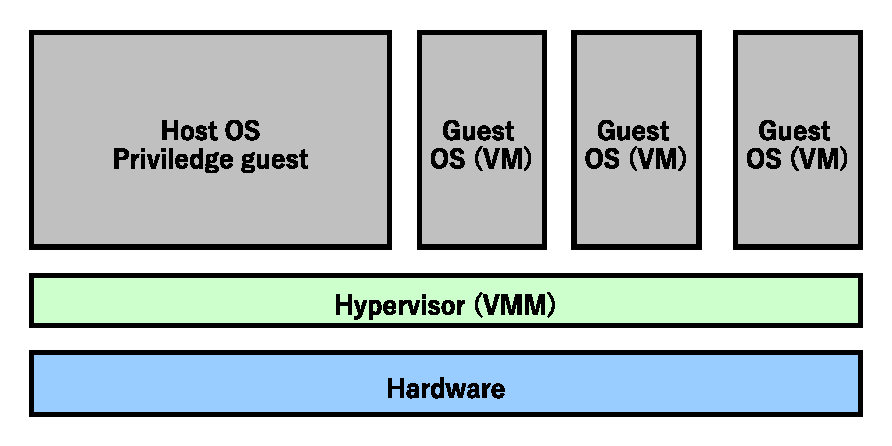
\includegraphics[scale=0.65]{fig02/paravirtualization.pdf}
    \caption{Paravirtualization architecture}
    \label{fig:paravirtualization}
\end{figure}


\subsection{Advantages of server virtualization}
Server virtualization is not just for big companies. \acrshort{sme}s can also take advantage of this technology, the advantages of which are presented here.

\paragraph{Reduced physical servers.} The first benefit of server virtualization is that since many virtual machines can run on a single physical server, the number of servers to buy and maintain will be reduced. With a traditional \acrshort{it} infrastructure, many servers are oversized in order to cope with possible peak loads. Combining multiple virtual machines in one place, a virtualized server is better exploited. The total number of machines required for the smooth functioning of the \acrshort{is} can thus be revised downwards.

\paragraph{Better availability.} Server virtualization solutions now allow the migration of virtual machines which is the process to move a virtual machine from one physical server to another without even needing to stop it \citep{livemigration,livemigration2}. This feature is a key element in improving the availability of services. The use of two physical servers thus makes it possible to easily double a virtualized infrastructure (redundancy). In case of a failure of one of the two servers, the virtual machines will be automatically moved to the second.

\paragraph{Better performance.} Another advantage of hot-migrating virtual machines between physical servers is that they can be used to distribute the workload between servers \citep{livemigration,livemigration2}. When a virtual machine rises to extreme load, others will be able to move to a less demanding physical server. Critical tasks will also work within a virtual machine that has more virtual \acrshort{cpu}, virtual \acrshort{ram} and virtual hard disk cores than the others. It is thus possible to modulate the size of the virtual machines according to the tasks they will have to perform.

\paragraph{Security enhanced.} In a traditional \acrshort{vse}/\acrshort{sme} \acrshort{it} infrastructure, \acrshort{erp}, file sharing, the mailing system, or even the web server, all run on the same server. However, if the mailing system is infected with a malware, all applications hosted on the machine are endangered. Server virtualization can be used to separate the different tasks of a physical server into many separate virtual machines, which will then be isolated from each other, thus dividing the services.

\paragraph{Anti-obsolescence warranty.} A part of an \acrshort{is}, for example, an \acrshort{erp}, is likely to work on a dedicated server, due to a specific configuration. Ensuring the renewal of this dedicated server, which is used by only one application, is often not very profitable. \acrshort{p2v} tools make it possible to transform most physical servers into virtual machines. Once this is done, the virtualized \acrshort{erp} server will be able to switch from an end-of-life machine to a new server by simply migrating the virtual machines.

\paragraph{Gain on licensing costs.} One operating system license per server is required. However, virtualization sometimes allows you to take advantage of license packs covering the OS of the physical server and its virtual machines. For existing virtual machines, it will not be necessary to repay a license when the physical server running them is changed. A plus, which also applies to applications running within these virtual machines.

\paragraph{Simplified backups.} With a virtualized infrastructure, the physical server is the only one physically present in the engine room. Virtual machines are pure software. This aspect greatly simplifies data backup operations. It is indeed possible to directly perform a backup of the contents of the virtual hard disk of a virtual machine. And even during its operation, by creating a snapshot of the virtual machine and its data. In case of a problem, this snapshot will restart the virtual machine in a previous state.


\paragraph{\gls{brp} easier to manage \citep{vttools}.} Virtualization can simplify the \glspl{brp}, making it easy to implement complex recovery plans. For example, launching a database server before the \acrshort{erp} server that accesses it. 


\paragraph{Test without paying.} Virtualization allows you to create a blank virtual machine in minutes. As long as your physical server does not display full, it will be possible to add new virtual machines to manage. Developers or system administrators will be able to exploit this feature to try new services without spending a single coin. Where a test server was previously needed, a simple virtual machine on an existing server of the company is enough today.

\paragraph{A stepping stone to the private cloud \citep{vttools}.} Server virtualization allows you to deploy new services within your computer system in the form of virtual machines. But also to dimension these virtual machines according to the criticality and the expected use. From there, why not offer a catalog of services and sizes of virtual machines to your business teams? And turn your \acrshort{it} into a service center. 

\subsection{Some server virtualization systems}

In the table \ref{table:virtualtools}, we compare some server virtualization systems based on their characteristics. 

\begin{table}[!h]
\ra{1.3}
    \centering
    \caption{Comparison of virtualization tools based on different factors}
    \begin{tabular}{p{5cm}>{\centering\arraybackslash}p{4cm}>{\centering\arraybackslash}p{4cm}}
     \toprule
     \textbf{Virtualization tools} & \textbf{License} & \textbf{Mode supported} \\
     \myrowcolour
     Bosch &  \gls{ops} & OS level \\
     KVM & \gls{ops} & Full \\
     \myrowcolour
     LXC & \gls{ops} & OS level \\
     Microsoft Virtual \acrshort{pc} & Commercial & Full \\
     \myrowcolour
     Parallels & Commercial & Full \\
     QEMU & \gls{ops} & Full \\
     \myrowcolour
     VMWare Vcenter & Commercial & Full \\
     VMWare Workstation & Free (not \glspl{ops}) & Full \\
     \myrowcolour
     VNUML (Virtual Network User Model Linux) & \gls{ops} & Full \\
     VServer & \gls{ops} & Para \\
     \myrowcolour
     Xen & \gls{ops} & Para \\
 
     \bottomrule
    \end{tabular}
    \label{table:virtualtools}
\end{table}

\section{\acrshort{numa} architecture}
 When using a server virtualization tool on a physical machine, for better configurations, it is essential to understand and master its architecture. Here we will try to give an outline of \acrshort{numa} architectures and present its impact on the performance of applications.
 
\par For the past decade, processor clock speed has increased dramatically. A multi-gigahertz \acrshort{cpu}, however, needs to be supplied with a large amount of memory bandwidth to use its processing power effectively. Even a single \acrshort{cpu} running a memory-intensive workload, such as a scientific computing application, can be constrained by memory bandwidth.This problem is amplified on \acrshort{smp} systems, where many processors must compete for bandwidth on the same system \glspl{bus}. Some high-end systems often try to solve this problem by building a high-speed data bus. However, such a solution is expensive and limited in scalability.

\paragraph{} \acrshort{numa} is an alternative approach that links several small, cost-effective nodes using a high-performance connection \citep{vttools2}. Each \textbf{node} contains processors\footnote{The group of processors in a node is usually called \textbf{socket}} and memory, much like a small \acrshort{smp} system. However, an advanced memory controller allows a node to use memory on all other nodes, creating a single system image as shown on Figure \ref{fig:numa_architecture}. When a processor accesses memory that does not lie within its own node (remote memory), the data must be transferred over the NUMA connection, which is slower than accessing local memory. Memory access times are not uniform and depend on the location of the memory and the node from which it is accessed, as the technology's name implies. 

\paragraph{} A lot of work was done to optimize existing algorithms to take into account \acrshort{numa} \citep{numa01,numa02,numa03}, this work led to many changes in existing \acrshort{os} to take into account \acrshort{numa}. \acrshort{numa} is relevant to multiple processors and means that memory can be accessed \textit{quicker if it is closer}. This means that memory is commonly \textbf{partitioned} at the hardware level in order to provide each processor in a multi-\acrshort{cpu} system with its own memory. The idea is to avoid an argument when processors attempt to access the same memory. This is a good thing and means that \acrshort{numa} has the potential to be more scalable than a \textbf{\acrshort{uma}} (multiple sockets share the same bus) design, particularly when it comes to environments with a large number of logical cores. 

\paragraph{}

\begin{figure}
    \centering
    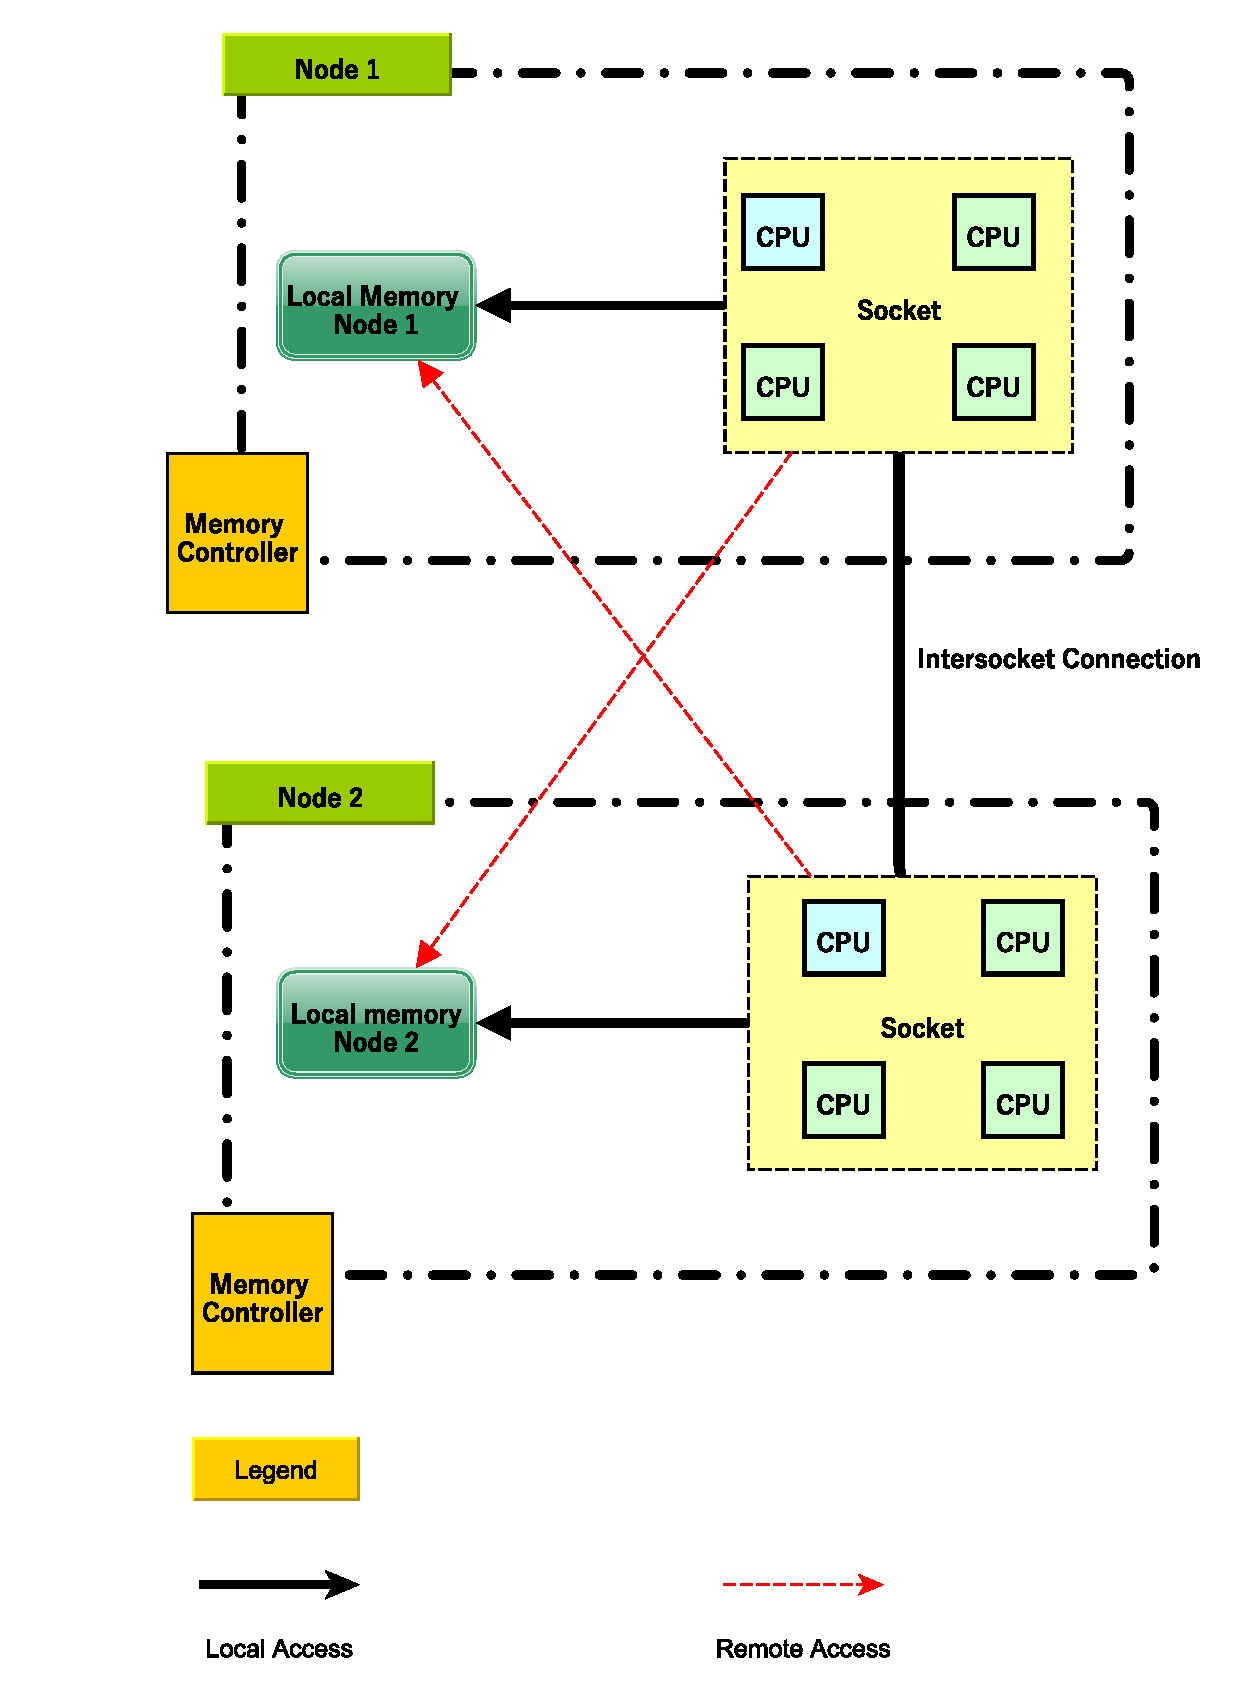
\includegraphics[scale=0.40]{fig02/numa-architecture.pdf}
    \caption{An example of a numa architecture}
    \label{fig:numa_architecture}
\end{figure}

\par Now that we have a good idea of what is concretely server virtualization, and the predominant architecture in \glspl{dc}s, let us present how our server virtualization system handle \acrshort{io} tasks for the virtual machines to helps us better understand the role played by the privileged domain (here the dom0) in these crucial tasks.

\section{\acrshort{io} mechanism in Xen}
\acrshort{io} tasks are handled by physical devices on a native \acrshort{os}. There are two major types of \acrshort{io} activities, \textbf{block and network \acrshort{io}} which use the block devices and network card by the means of \glspl{dd}s. How the virtualization system Xen manages virtual devices will be the point of interest in this section.

\paragraph{} Virtual devices under Xen are provided by a \textbf{split device driver model}. The illusion of the virtual device is provided by two co-operating drivers: the \textbf{front-end}, which runs in the unprivileged domain and the \textbf{back-end}, which runs in the privileged domain (here the domain0) as shown on Figure \ref{fig:split-model}. The front-end driver appears to the unprivileged guest as if it was a real device, for instance, a block or network device. It receives \acrshort{io} requests from its kernel, as usual. However, since it does not have access to the physical hardware of the system it must then issue requests to the back-end. 

\begin{figure}[!h]
    \centering
    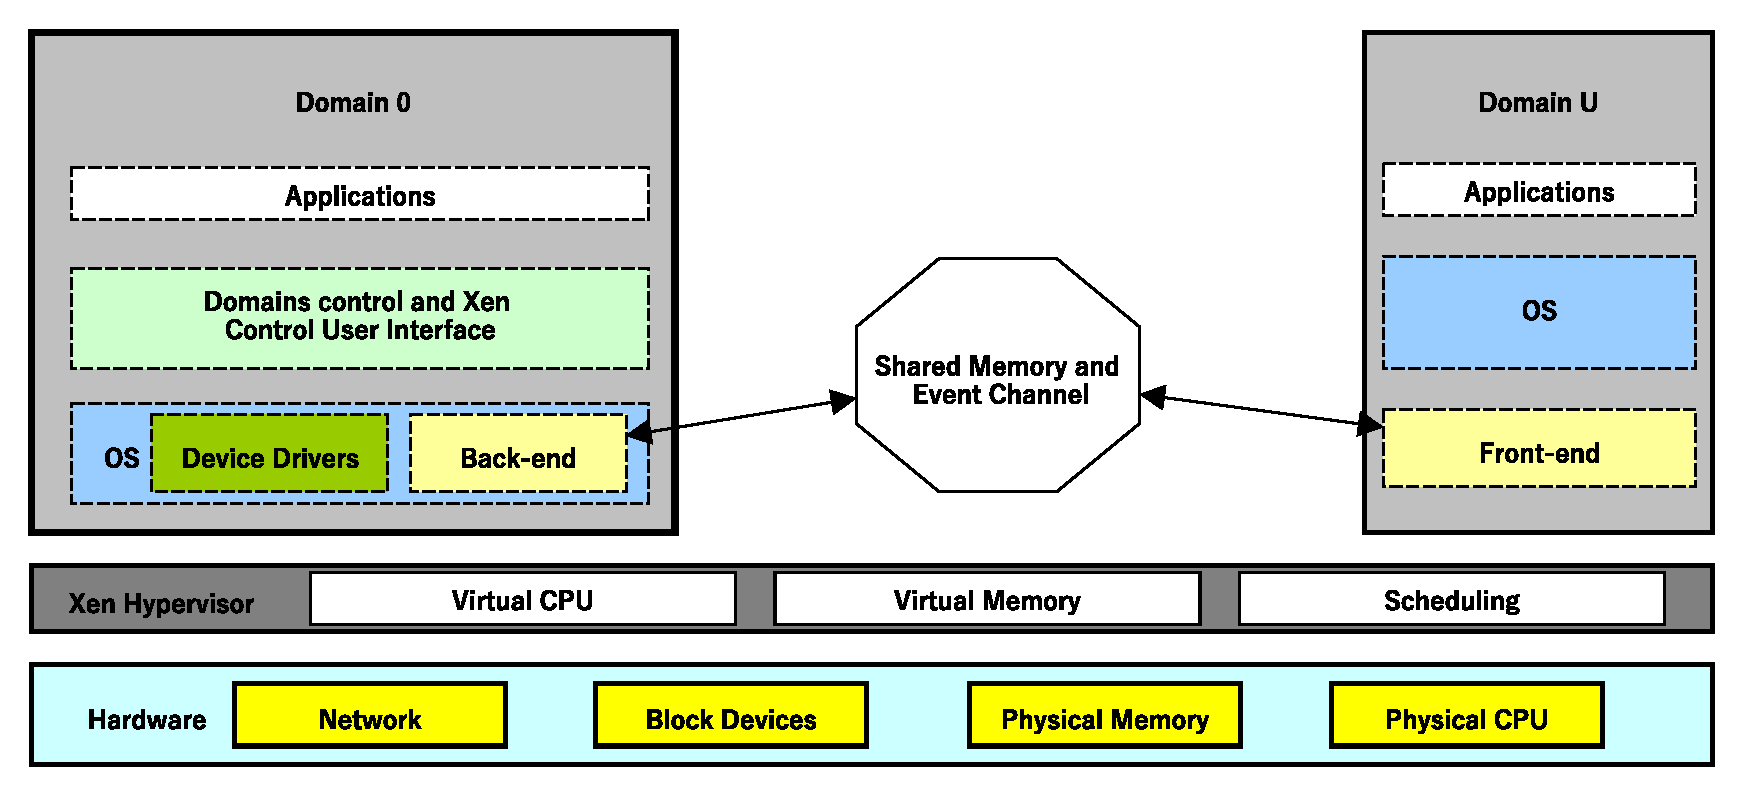
\includegraphics[width=\linewidth]{fig02/split-driver.pdf}
    \caption{Split driver model}
    \label{fig:split-model}
\end{figure}

\paragraph{} The backend driver is responsible for receiving these \acrshort{io} requests, \textbf{verifying} that they are safe and then issuing them to the \textbf{real device} hardware. The back-end driver appears to its kernel as a normal user of in-\glspl{kernel} \acrshort{io} functionality. When the \acrshort{io} completes the back-end notifies the front-end that the data is ready for use, the front-end is then able to report \acrshort{io} completion to its own \glspl{kernel}. Split drivers exchange requests and responses in \textbf{shared memory}, with an \textbf{event channel} for asynchronous notifications of activity \citep{xen_book}. When the front-end driver comes up, it uses the \textbf{Xenstore} to set up a shared memory frame and an interdomain event channel for communications with the backend. Once this connection is established, the two can communicate directly by placing requests/responses into shared memory and then sending notifications on the event channel. In the sections below, we will detail what happens in the case of block \acrshort{io} and network \acrshort{io}.

\subsection{Network \acrshort{io} mechanism}
From the point of view of the back-end domain itself, the network back-end driver consists of a number of ethernet devices. Each of these has a logical direct connection to a virtual network device in another domain. This allows the back-end domain to route, bridge, firewall, etc the traffic to/from the other domains using normal operating system mechanisms \citep{xen_book}. Corresponding to each virtual interface in a guest domain, a back-end interface is created in the driver domain, which acts as the proxy for that virtual interface in the driver domain (dom0). Each virtual interface uses two \textbf{descriptor rings} (two shared memory rings), one for transmitting, the other for receiving. Each descriptor identifies a block of contiguous machine memory allocated to the domain. Each back-end interface has a number of \textbf{queues} to handle requests from a virtual interface.

\subsubsection{Packet transmission}

As shown on Figure \ref{fig:transmit_io}, the transmit ring carries packets to transmit from the guest to the back-end domain. By doing so,

\begin{itemize}
    \item it writes/copies the packet in the transmit ring (which is a shared memory between the driver domain and the virtual guest),
    \item then generates a virtual \glspl{interrupt} request (VIRQ) to notify the driver domain (dom0)
    \item and the return path of the transmit ring carries messages indicating that the contents have been physically transmitted and the backend no longer requires the associated memory pages.
\end{itemize}

\begin{figure}[!h]
    \centering
    \includegraphics[scale=0.65]{fig02/transmit_io.png}
    \caption{Network I/O transmit mechanism between front-end and back-end}
    \label{fig:transmit_io}
\end{figure}

Each transmit request is followed by a transmit response at some later date. This is part of the shared-memory communication protocol and allows the guest to (potentially) retrieve internal structures related to the request.

\subsection{Packet reception}
To receive packets, the guest places descriptors of unused pages on the receive ring. The back-end will return received packets by exchanging these pages in the domain's memory with new pages containing the received data and passing back descriptors regarding the new packets on the ring. This zero-copy approach as shown on Figure \ref{fig:zero_copy}, allows the back-end to maintain a pool of free pages to receive packets into, and then deliver them to appropriate domains after examining their headers. Receive requests must be queued by the front-end, accompanied by a donation of page-frames to the back-end. The back-end transfers page frames full of data back to the guest. Receive response descriptors are queued for each received frame.

\paragraph{} Guests are expected to return memory to the hypervisor in order to use the network interface. They must do this or they will exceed their maximum memory reservation and will not be able to receive incoming frame transfers. When necessary, the back-end is able to replenish its pool of free network buffers by claiming some of this free memory from the hypervisor.

\begin{figure}[!h]
    \centering
    \includegraphics[scale=0.65]{fig02/zero_copy.png}
    \caption{Zero copy mechanism}
    \label{fig:zero_copy}
\end{figure}



\subsection{Block \acrshort{io} mechanism}
All guest \acrshort{os} disk access goes through the \textbf{virtual block device} (VBD) interface. This interface allows domains access to portions of block storage devices visible to the block back-end device. The VBD interface is a split driver, similar to the network interface described above. A single shared memory ring is used between the front-end and back-end drivers for each virtual device, across which \acrshort{io} requests and responses are sent. Any block device accessible to the back-end domain can be exported as a VBD. Each VBD is mapped to a device node in the guest, specified in the guest's startup configuration.

\paragraph{} The per-(virtual)-device ring between the guest and the block back-end supports two messages:

\begin{itemize}
    \item \textbf{READ}: Read data from the specified block device. The front end identifies the device and location to read from and attaches pages for the data to be copied to (typically via \acrshort{dma} from the device). The back-end acknowledges completed read requests as they finish.
    \item \textbf{WRITE}: Write data to the specified block device. This functions essentially as READ, except that the data moves to the device instead of from it.


\end{itemize}


In the next chapter, we will discuss about the questions raised in the problematic and its assessment.
